\documentclass[11pt]{article}
\usepackage[margin=1in]{geometry}
\usepackage{volfit_preamble}
\graphicspath{{figures/}}

\title{\textbf{The Calibration Objective}\\[2pt]
\large Vega-normalized residuals, observation weighting, bid--ask bands, and fit quality\\[2pt]
\normalsize Vol-Fitter Technical Notes, No.~07}
\author{Vol-Fitter}
\date{\today}

\begin{document}
\maketitle
% Auto-generated by gen_objective.py — do not edit.
\newcommand{\objwingratio}{1.3}
\newcommand{\objroughmid}{0.1}
\newcommand{\objroughband}{0.1}
\newcommand{\objmidanchor}{0.05}


\begin{abstract}
Every model in the Vol-Fitter --- LQD, SVI, Multi-Core Sigmoid (MCS), local volatility ---
is calibrated by minimizing the \emph{same} kind of objective, and this note
documents that shared machinery so the model notes need not repeat it. Three
ingredients: a residual \emph{scale} (vega-normalized price, so the loss behaves
like a volatility error while every iterate stays a valid price); a per-quote
\emph{weight} (equal, or the density-corrected time-value weighting that prevents
a dense strike cluster from dominating a sparse but informative wing); and a
\emph{target} (the mid, or a bid--ask/haircut band that lets the fit sit anywhere
inside the quoted spread and only resists leaving it). We give the weighting
formula and its uniform-grid sanity check, the squared-hinge band objective with
its small mid anchor and its space-agnostic design, and the goodness-of-fit
metric that reports the \emph{actual} calibrated misfit rather than a decorative
RMS. Figures generated by the production calibrator show the density correction
re-balancing weight from the ATM cluster toward the wings, and a band fit relaxing
the pull toward noisy mids.
\end{abstract}

\tableofcontents
\newpage

%======================================================================
\section{The residual scale: vega normalization}
\label{sec:vega}

A smile is quoted in volatility but priced in price, and the two have very
different scales across moneyness: a vol bp in the wings is worth a tiny fraction
of a vol bp ATM in price terms. The Vol-Fitter resolves this once, for all models,
by working in \emph{vega-normalized price} residuals. For a quote at $k$ with
total variance $w$, the residual is
\begin{equation}
r=\frac{C^{\text{model}}(k)-\Black(k,w)}{\partial_\sigma\Black(k,w)+\eta},
\qquad \partial_\sigma\Black=\phin(d_+)\sqrt T,
\label{eq:vega}
\end{equation}
with a small vega floor $\eta$ in the far wings. The numerator is computed in the
model's native, arbitrage-preserving price space (so every iterate is a valid
density); the division by vega undoes the price-to-vol scale, so the optimizer
sees something close to a uniform volatility error.

\begin{heuristic}
Why not just fit volatility directly? Because for the density-based models
(LQD, LV) the \emph{price} is the arbitrage-free object and the implied vol is a
nonlinear read-off; fitting price keeps the feasible set convex-clean, and the
vega division recovers the vol-like loss for free. For the vol-space models
(SVI, MCS) the residual is already a vol error and \eqref{eq:vega} degenerates to
exactly that. One residual concept, two implementations, identical units.
\end{heuristic}

\begin{invariant}
\begin{enumerate}[leftmargin=1.6em]
\item One objective vocabulary for every model: same residual units, same
weight schemes, same band construction --- a mode or scheme change means the
same thing on LQD, SVI, MCS and LV.
\item Weights are mean-normalized to one, so switching schemes never silently
re-tunes the data-versus-regularization balance.
\item Inside the quoted band the fit pays only the small mid anchor ---
the band never pushes, it only stops punishing.
\item The reported RMS is the distance to the objective that was actually
minimized, under the weights that were actually used.
\end{enumerate}
\end{invariant}

%======================================================================
\section{Observation weighting}
\label{sec:weights}

\subsection{The problem with counting quotes}

Each squared residual enters the loss with a weight $\omega_i$. With equal weights
the fit is driven by wherever the quotes happen to be \emph{dense} --- typically a
tight ATM cluster --- so an isolated but economically important wing quote barely
registers. The desk wants the opposite: weight should follow the \emph{economic}
importance of a strike, not the accident of how finely it was sampled.

\subsection{Density-corrected time-value weights}

The Vol-Fitter offers two schemes via \texttt{weightScheme}. The default
\texttt{equal} uses unit weights. The \texttt{tv\_density} scheme implements
\begin{equation}
\boxed{\;\omega_i=\max(\mathrm{TV}_i,\eps)\,\frac{s_i}{\bar s},\;}
\label{eq:tvweights}
\end{equation}
where $\mathrm{TV}_i$ is the quote's \emph{time value} (its OTM option price, which
in forward-normalized units is its whole value), and $s_i$ is the one-dimensional
Voronoi cell width of the quote in log-strike: the stretch of the strike axis
closer to this quote than to any other --- half the gap to each neighbour,
one-sided at the ends --- i.e.\ how much strike range this quote alone covers.
The factor $\mathrm{TV}_i$ is the economic weight (a quote
on a richly-priced option matters more); the factor $s_i/\bar s$ is the
\emph{density correction}, dividing out the exchange's listing density $1/s_i$ so
that the \emph{aggregate} weight over strike space follows the time-value measure
$\mathrm{TV}(x)\,\dd x$ rather than the raw quote histogram --- without it, the
densely-listed ATM cluster would outvote the wings simply by quote \emph{count}.

\begin{proposition}[Uniform-grid sanity check]
On a uniform log-strike grid all $s_i$ are equal, so $s_i/\bar s=1$ and
\eqref{eq:tvweights} reduces to $\omega_i=\mathrm{TV}_i$ --- the pure time-value
weighting, with no double-counting to correct.
\end{proposition}

A cap \texttt{DEFAULT\_MAX\_MULT}$=10$ on the spacing multiplier $s_i/\bar s$
stops a single isolated far-wing quote from dominating. Crucially the weights are
\emph{mean-normalized to one}, so switching schemes leaves the
data-versus-regularization balance unchanged: the LQD ridge, the MCS hat
ridge and the LV roughness penalty are all tuned against unit-mean weights and
never silently over- or under-regularize when the scheme changes.

\Cref{fig:weights} shows the effect on a non-uniform strike set with a dense ATM
region and sparse wings: the dense ATM quotes are individually \emph{down}-weighted
and the sparse wing quotes \emph{up}-weighted relative to equal, re-balancing the
fit toward the full strike range while still respecting that ATM options carry
more time value (the net wing-to-ATM weight ratio here is $\objwingratio$).

\begin{figure}[H]
\centering
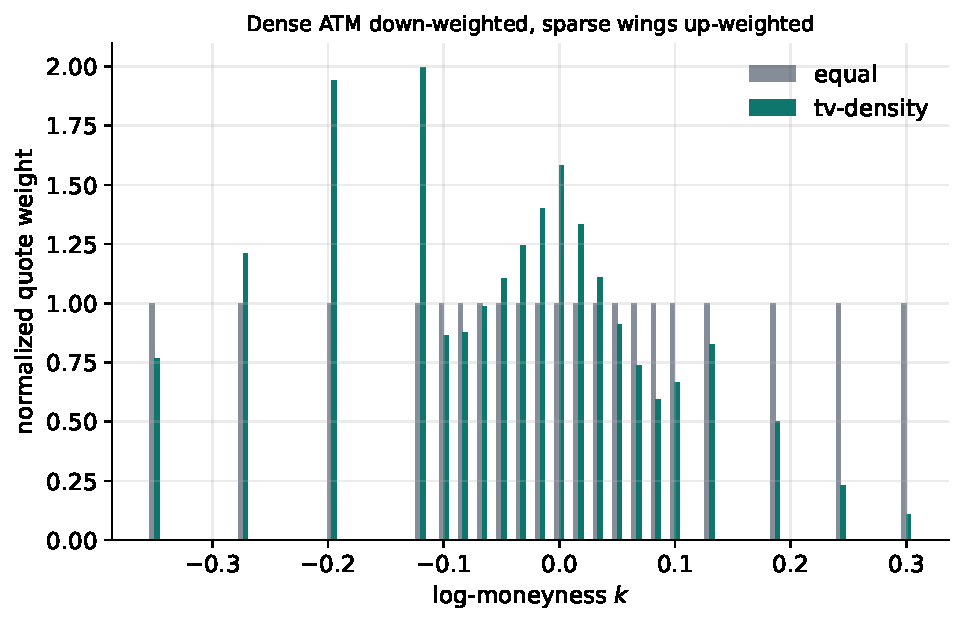
\includegraphics[width=0.78\textwidth]{fig_obj_weights.pdf}
\caption{Equal vs density-corrected time-value weights on a non-uniform strike
set. The dense ATM cluster is down-weighted per quote, the sparse wings
up-weighted, so the aggregate weight follows the time-value measure rather than
the quote histogram.}
\label{fig:weights}
\end{figure}

%======================================================================
\section{Bid--ask bands}
\label{sec:band}

\subsection{Why a band, not a mid}

A mid quote pretends a price is known exactly; a real quote is a \emph{band}
$[\text{bid},\text{ask}]$, and any curve inside it is consistent with the market.
Fitting the mid forces the curve to chase the midpoint of every spread, including
the noise in illiquid wings where the spread is wide. The band objective instead
penalizes only \emph{leaving} the band, with a gentle pull toward mid for
identifiability:
\begin{equation}
\boxed{\;\text{loss}_i=\max(m_i-\text{hi}_i,0)^2+\max(\text{lo}_i-m_i,0)^2
+\theta_{\text{mid}}\,(m_i-\text{mid}_i)^2,\;}
\label{eq:band}
\end{equation}
where $m_i$ is the model value, $[\text{lo}_i,\text{hi}_i]$ the (possibly
haircut-adjusted) band, and $\theta_{\text{mid}}=\objmidanchor$ the mid-anchor
weight. Inside the band the first two terms vanish: the fit is \emph{free}, paying
only the small anchor; once it leaves, the squared hinge pulls it back hard.

\subsection{Modes and the haircut}

Three modes via \texttt{fitMode}. \texttt{mid} sets
$\text{lo}=\text{hi}=\text{mid}$ (the band collapses, recovering a mid fit).
\texttt{bidask} uses the raw $(\text{bid},\text{ask})$. \texttt{haircut} tightens
each side toward mid by \texttt{haircut} volatility points, never crossing mid,
\begin{equation}
\text{lo}=\min(\text{bid}+h,\text{mid}),\qquad
\text{hi}=\max(\text{mid},\text{ask}-h),
\end{equation}
so a quote tighter than $2h$ collapses gracefully to a mid fit on that strike.
This makes the haircut one dial that spans the whole mid-to-band spectrum: tight
ATM spreads collapse onto the mid (the fit follows mids exactly where they are
informative), while wide wing spreads keep a meaningful band (the fit only has to
stay inside it). The
hinge is monotone in the quote value, so the \emph{same} construction works in any
monotone residual space --- implied vol for SVI/MCS, vega-normalized price for
LQD/LV --- and the band-violation subgradient $\sgn$ feeds the analytic Jacobians.
Both are one line:

\begin{lstlisting}[caption={The two-sided band hinge and its subgradient (from
\texttt{calib/band.py}; match production exactly).},label={lst:band}]
def band_violation(model, lo, hi):   # > 0 only outside [lo, hi]; 0 inside
    return np.maximum(model - hi, 0.0) + np.maximum(lo - model, 0.0)

def band_violation_sign(model, lo, hi):   # +1 above, -1 below, 0 inside
    return np.where(model > hi, 1.0, 0.0) - np.where(model < lo, 1.0, 0.0)
\end{lstlisting}

\Cref{fig:band} shows a band fit against a mid fit on a smile with a widening wing
spread and noisy mids: the band fit is content to sit anywhere inside the shaded
band, relaxing the pull toward the noisy midpoints, while the mid fit is anchored
to each midpoint.

\begin{figure}[H]
\centering
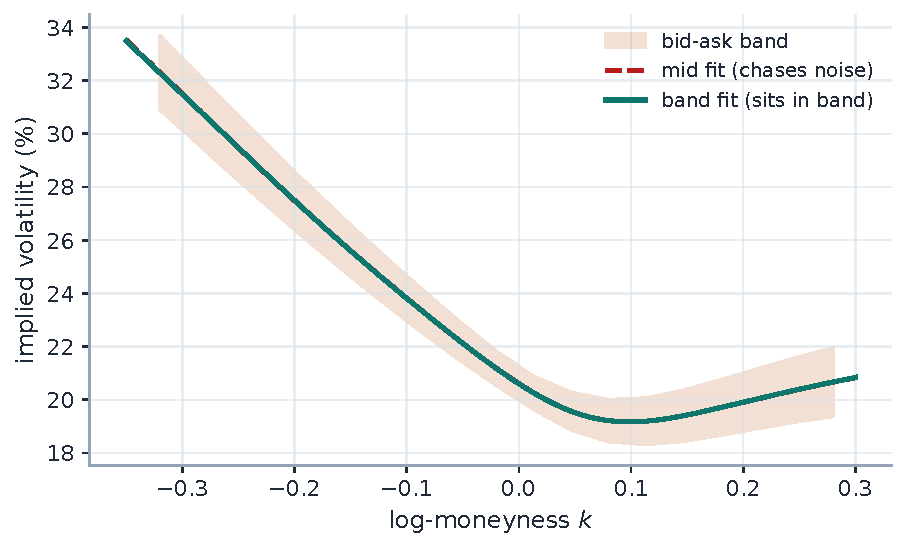
\includegraphics[width=0.78\textwidth]{fig_obj_band.pdf}
\caption{A bid--ask band fit (solid) vs a mid fit (dashed) with the quoted band
shaded. Inside the band the fit pays only the small mid anchor, so it need not
chase noisy midpoints --- most valuable in wide-spread wings.}
\label{fig:band}
\end{figure}

\begin{heuristic}
The band's value scales with model flexibility. A rigid parametric model (a
seven-parameter LQD) already smooths through mid noise, so the band and mid fits
nearly coincide; a flexible model (a many-vertex local-vol surface) can be pulled
into spurious wiggles by noisy mids, and there the band's freedom-to-sit-anywhere
is what keeps the surface smooth. The band is a \emph{regularizer that costs no
bias}: it does not push the fit anywhere, it merely stops penalizing it for being
inside the spread.
\end{heuristic}

%======================================================================
\section{Goodness of fit}
\label{sec:rms}

A reported fit error should reflect the \emph{objective that was minimized}, not a
decorative quantity. The Vol-Fitter's weighted RMS therefore mirrors the active
configuration: the distance to the fit \emph{target} (mid, or band violation, so a
fit sitting happily inside the band reports near-zero error even if it is far from
mid), under the active \emph{weighting} scheme, including the var-swap penalty term
when active. It is returned as a $(\sum\omega r^2,\sum\omega)$ pair so node errors
aggregate correctly into a surface RMS. This is why the same surface can report a
different RMS under \texttt{mid} and \texttt{bidask}: the two minimize different
objectives, and the metric is honest about which.

%======================================================================
\section{What is original here}
\label{sec:original}

The vega normalization is standard; the contributions are the
\emph{density-corrected} weighting \eqref{eq:tvweights} --- separating economic
importance (time value) from sampling density (Voronoi spacing), with the
mean-normalization that keeps regularization invariant across schemes --- and the
\emph{space-agnostic squared-hinge band} \eqref{eq:band} whose monotone subgradient
plugs into every model's analytic Jacobian, so bid--ask fitting is a first-class
mode rather than a bolt-on. Together they let the desk express ``fit what matters,
to within the spread'' in two orthogonal knobs.

%======================================================================
\section{Traceability}
\label{sec:traceability}

\begingroup
\small
\setlength{\tabcolsep}{3pt}
\begin{longtable}{@{}p{0.32\textwidth}p{0.11\textwidth}p{0.24\textwidth}p{0.29\textwidth}@{}}
\caption{Claims in this note and the code/tests that lock them.}\\
\toprule Claim & Object & Code anchor & Test anchor\\ \midrule
\endfirsthead
\toprule Claim & Object & Code anchor & Test anchor\\ \midrule
\endhead
Density-corrected weights match the design note's worked example &
\eqref{eq:tvweights} &
\nolinkurl{calib/weights.py} &
\nolinkurl{test_weights.py::test_doc_worked_example}\\
Uniform grid reduces to pure time value &
\cref{sec:weights} &
\nolinkurl{calib/weights.py} &
\nolinkurl{test_weights.py::test_uniform_grid_reduces_to_time_value}\\
Dense cluster down-weighted; mean-one normalization &
\eqref{eq:tvweights} &
\nolinkurl{calib/weights.py::resolve_weights} &
\nolinkurl{test_weights.py::test_dense_region_downweighted}, \nolinkurl{::test_resolve_weights_equal_is_none_and_tv_is_mean_one}\\
The scheme moves every model &
invariant~1 &
\nolinkurl{calib/weights.py} &
\nolinkurl{test_weights.py::test_weight_scheme_moves_every_model}\\
Band modes; haircut collapses gracefully to mid &
\cref{sec:band} &
\nolinkurl{calib/band.py::resolve_band} &
\nolinkurl{test_band_fit.py::test_resolve_band_modes}, \nolinkurl{::test_haircut_default_is_half_vol_point}\\
Zero residual inside the band &
\eqref{eq:band} &
\nolinkurl{calib/band.py} &
\nolinkurl{test_band_fit.py::test_band_residuals_zero_inside_band}\\
RMS mirrors the minimized objective &
\cref{sec:rms} &
\nolinkurl{calib/rms.py} &
\nolinkurl{test_rms.py::test_mid_mode_is_weighted_rms_distance_to_mid}, \nolinkurl{::test_band_mode_zero_inside_band_distance_outside}\\
Band-mode RMS never exceeds mid-mode; surface pooling &
\cref{sec:rms} &
\nolinkurl{calib/rms.py} &
\nolinkurl{test_rms.py::test_band_mode_rms_not_above_mid_mode}, \nolinkurl{::test_surface_rms_pools_expiries}\\
\bottomrule
\end{longtable}
\endgroup

\appendix
%======================================================================
\section{Hyperparameter atlas}
\label{app:atlas}

\begin{longtable}{p{0.26\textwidth}p{0.14\textwidth}p{0.52\textwidth}}
\caption{Calibration-objective hyperparameters.}\label{tab:atlas}\\
\toprule Knob & Default & Role\\ \midrule
\endfirsthead \toprule Knob & Default & Role\\ \midrule \endhead
\multicolumn{3}{l}{\emph{Surfaced (FitSettings / OptionsSettings)}}\\ \midrule
\texttt{weightScheme} & \texttt{equal} & \texttt{equal} or \texttt{tv\_density}.\\
\texttt{fitMode} & \texttt{mid} & \texttt{mid} / \texttt{bidask} / \texttt{haircut}.\\
\texttt{haircut} $h$ & $0.005$ & Haircut in vol points (each band side toward mid).\\
\texttt{midAnchorWeight} $\theta_{\text{mid}}$ & $\objmidanchor$ & Mid anchor strength vs band penalty ($=1$).\\
\midrule
\multicolumn{3}{l}{\emph{Hidden}}\\ \midrule
\texttt{DEFAULT\_MAX\_MULT} & $10$ & Cap on the Voronoi spacing multiplier $s_i/\bar s$.\\
$\eps$ & $10^{-12}$ & Floor on time value / spacing.\\
$\eta$ (vega floor) & $10^{-4}$ & Floor on Black vega in \eqref{eq:vega}.\\
\bottomrule
\end{longtable}

\noindent\textbf{Performance.} Weighting is $O(m\log m)$ (one sort) and the band
residual is $O(m)$, both negligible against the fit; the band subgradient is
analytic so it adds nothing to Jacobian assembly. Switching schemes or modes bumps
the options version and triggers exactly one refit.

%======================================================================
\section{Reference implementation: the band residual stack}
\label{app:ref}

The full objective stacks two blocks per quote: the band violation (scaled by the
per-quote weight, or $1/\text{vega}$ in the LQD/LV price space) and a weak mid
anchor of strength $\theta_{\text{mid}}$, so the fit is free inside the band yet
never drifts off a one-sided quote. Squaring and summing reproduces the loss
$\max(m-\text{hi},0)^2+\max(\text{lo}-m,0)^2+\theta_{\text{mid}}(m-\text{mid})^2$.
Matches production to $10^{-15}$.

\begin{lstlisting}[caption={The stacked band-objective residual (distilled from
\texttt{calib/band.py}).}]
def band_residuals(model, lo, hi, mid, scale, mid_anchor_weight):
    viol = scale * band_violation(model, lo, hi)         # push inside the bid/ask band
    anchor = np.sqrt(mid_anchor_weight) * scale * (model - mid)   # weak pull to mid
    return np.concatenate([viol, anchor])                # least-squares stack (length 2N)
\end{lstlisting}

\begin{thebibliography}{9}
\bibitem{tvweights} Vol-Fitter Technical Note, \emph{Density-corrected time-value
weights} (\texttt{Docs/iv\_time\_value\_density\_weights.tex}).
\bibitem{Gatheral2006} J.~Gatheral. \emph{The Volatility Surface}. Wiley, 2006.
\end{thebibliography}

\end{document}
